\documentclass{beamer}

\usepackage[utf8]{inputenc}
\usepackage[english]{babel}
\usepackage[T1]{fontenc}
%\usepackage{CJKutf8}
\usepackage{xcolor}
\usepackage{amsmath,amssymb}
\usepackage[overload]{empheq}
\usepackage{hyperref}
\usepackage{graphicx}
\usepackage{subcaption}
\DeclareMathOperator{\E}{\mathbb{E}}
\newcommand{\norm}[1]{\left\lVert#1\right\rVert}
\usepackage{xcolor}
\usepackage{subcaption}
\DeclareMathOperator*{\argmax}{arg\,max}
\DeclareMathOperator*{\argmin}{arg\,min}

\usepackage{xeCJK}
\setCJKmainfont[BoldFont=STZhongsong, ItalicFont=STKaiti]{STSong}
\setCJKsansfont[BoldFont=STHeiti]{STXihei}
\setCJKmonofont{STFangsong}

\usepackage{bbm}

\newtheorem{task}{Main problem}


\usetheme{Madrid}
\usecolortheme{seahorse}

%Information to be included in the title page:
\title[ImageSeg] %optional
{Image Segmentation and Clustering Techniques}

\subtitle{Statistical Computing midterm project}


\author[D.C.]
{Ding-Chih  Lin}


\institute[NTHU] % (optional)
{
National Tsing Hua University, Institute of Statistics
}

\date[May 11, 2021] % (optional)
{May 11, 2021}


\begin{document}

\AtBeginSection[]
{
    \begin{frame}
        \frametitle{Table of Contents}
        \tableofcontents[currentsection]
    \end{frame}
}


\frame{\titlepage}


\begin{frame}{Agenda}
\tableofcontents
\end{frame}


\section{Introduction}


\begin{frame}
\frametitle{Image segmentation}

\begin{description}
	\item[\textbf{Image Segmentation:}\hfill]
\end{description}

\begin{itemize}
	\item Partition a digital image into multiple segments
	\item Simplify the representation of an image into something which is meaningful
	\item Assign a label to every pixel in an image such that pixels with the same label shared certain characteristics.
\end{itemize}

\end{frame}

\begin{frame}
\frametitle{Practical applications}

\begin{columns}
	\column{0.55\linewidth}
	\begin{description}
		\item[\textbf{Practical applications:}\hfill]
	\end{description}
	\begin{itemize}
		\item Tumor segmentation from medical images
		\item Object detection for autonomous vehicles or satellites
		\item Color quantization
		\item Optical character recognition (OCR) 
	\end{itemize}
	\column{0.45\linewidth}
	\centering
		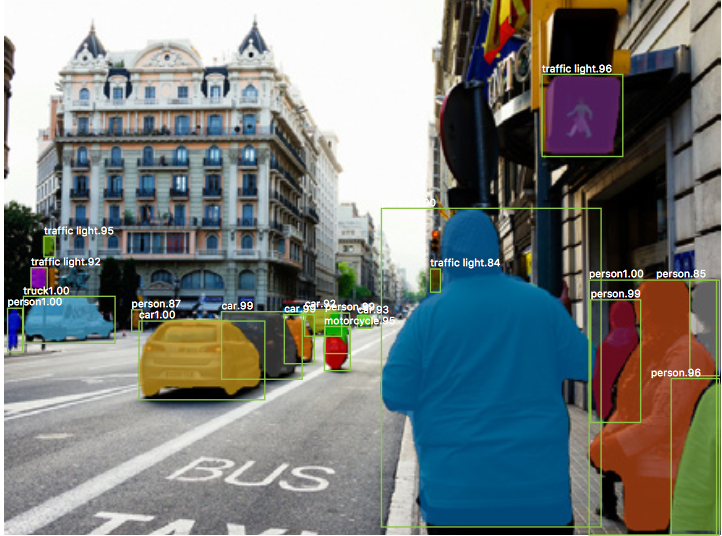
\includegraphics[height=4cm, width=5cm]{image/intro.png}
\end{columns}

\end{frame}


\section{Clustering Techniques}

\begin{frame}
\frametitle{Method 1: K-means clustering}

\begin{description}
	\item[\textbf{K-means Clustering:}\hfill]
\end{description}

\begin{itemize}
	\item \textit{Compactness}, cluster the objects which share lower distances
	\item Use \textit{random partition method} to decide initial centroids
	\item Utilize naive K-means algorithm
\end{itemize}

\end{frame}



\begin{frame}
\frametitle{Method 2: Spectral clustering}
\begin{description}
	\item[\textbf{Spectral Clustering:}\hfill]
\end{description}

\begin{itemize}
	\item \textit{Connectedness}, cluster the objects which are connected to each other
	\item Build a graph $G(V, E)$ with corresponding weights (similarity) $w_{ij}$
	\item Identify the clusters of nodes based on the edges connecting them
	\item Utilize information from the eigenvalues of the $W$ built from the graph
\end{itemize}

\end{frame}


\begin{frame}
\frametitle{Method 3: Hidden Markov Model}
\begin{description}
	\item[\textbf{Hidden Markov Model:}\hfill]
\end{description}

\begin{itemize}
	\item Discrete-time doubly embedded stochastic process
	\item Process $X$ being modeled is assumed to be a Markov process with unobserved states $Y$ that depends on $X$
	\item Learn about $X$ in order to observe or obtain $Y$
	\item Assume the emission probabilities are normally distributed
\end{itemize}

\end{frame}

\begin{frame}
\frametitle{Simulation Study}

\begin{figure}[h!]%
    \centering
    {\renewcommand{\arraystretch}{0}
    \begin{tabular}{c@{}c}
    \begin{subfigure}[b]{.55\columnwidth}
        \centering
        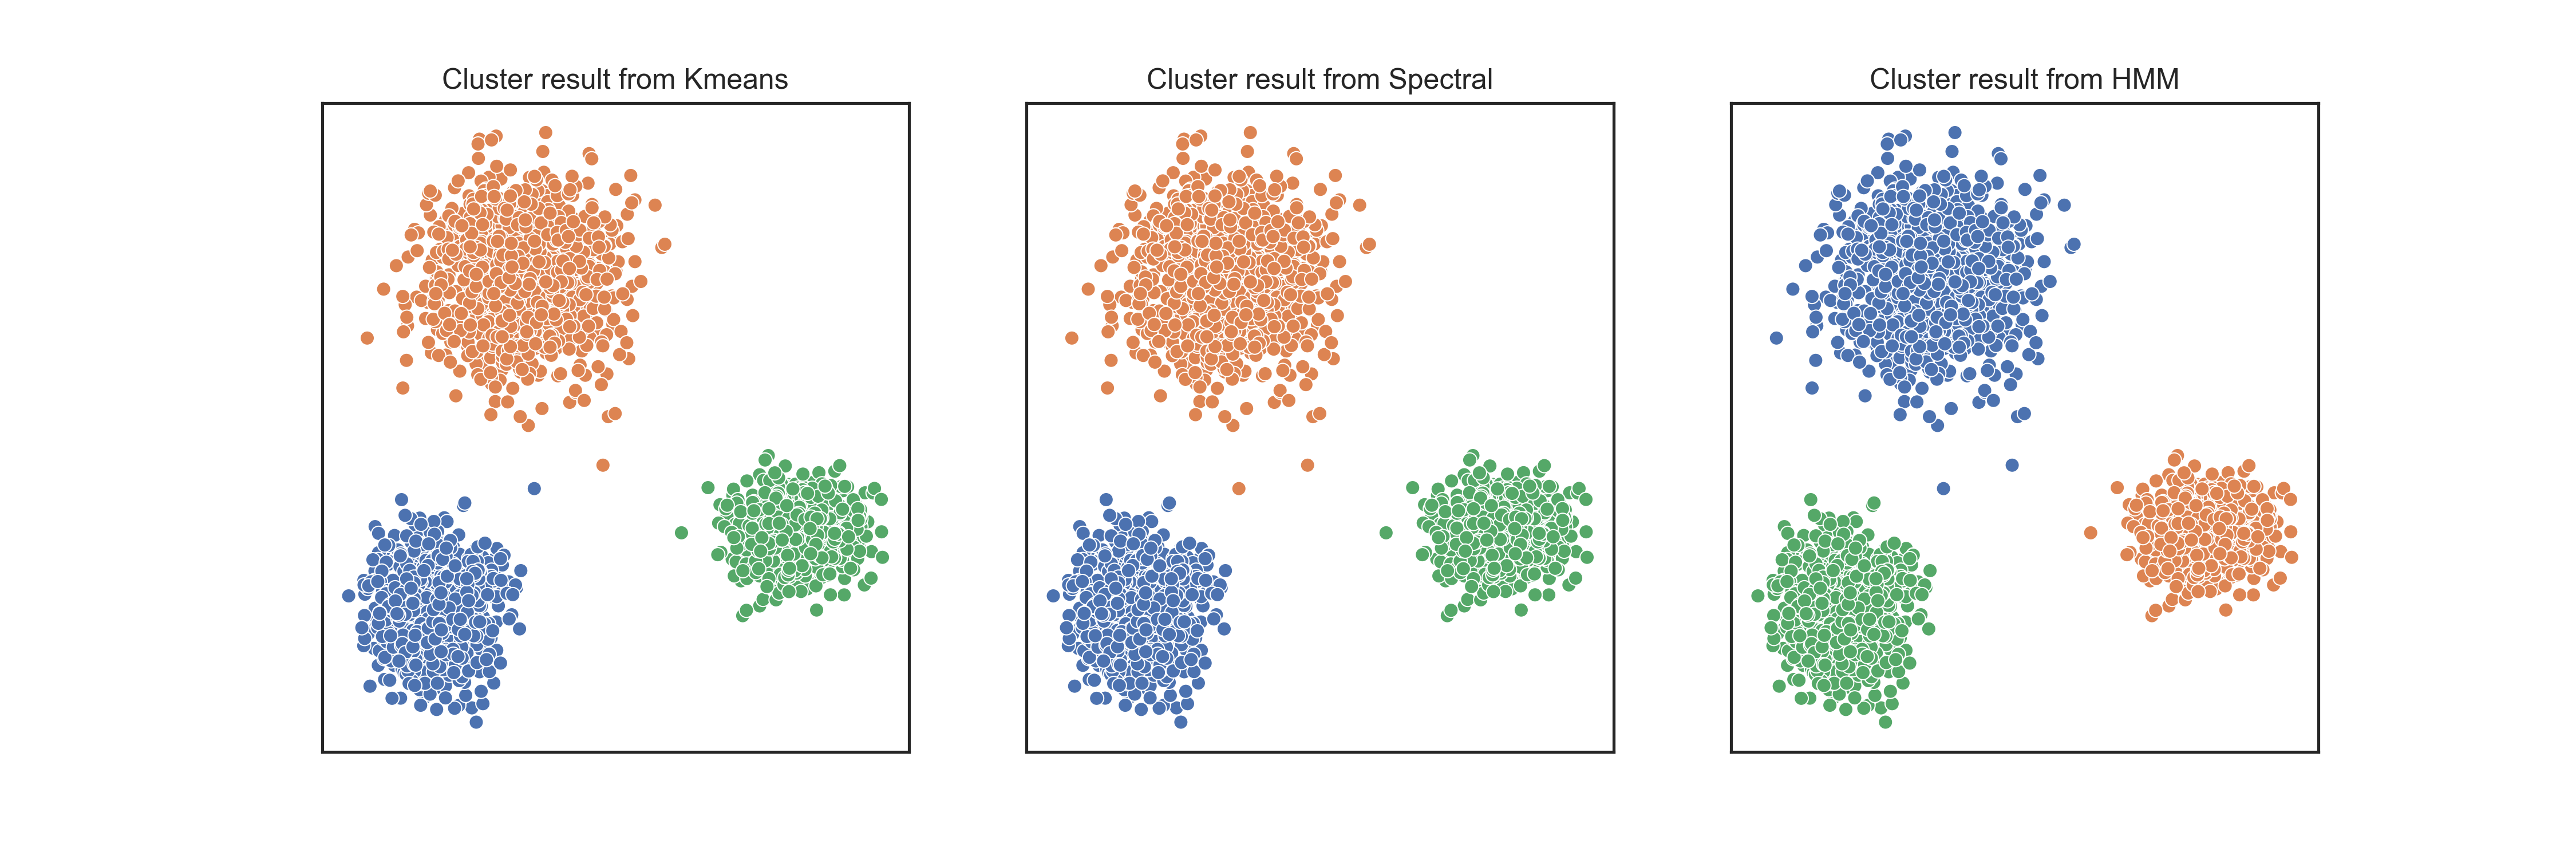
\includegraphics[width=\columnwidth]{../Simu_results/sen1_clust.png}%
    \end{subfigure}\\
    \begin{subfigure}[t]{.55\columnwidth}   
        \centering 
        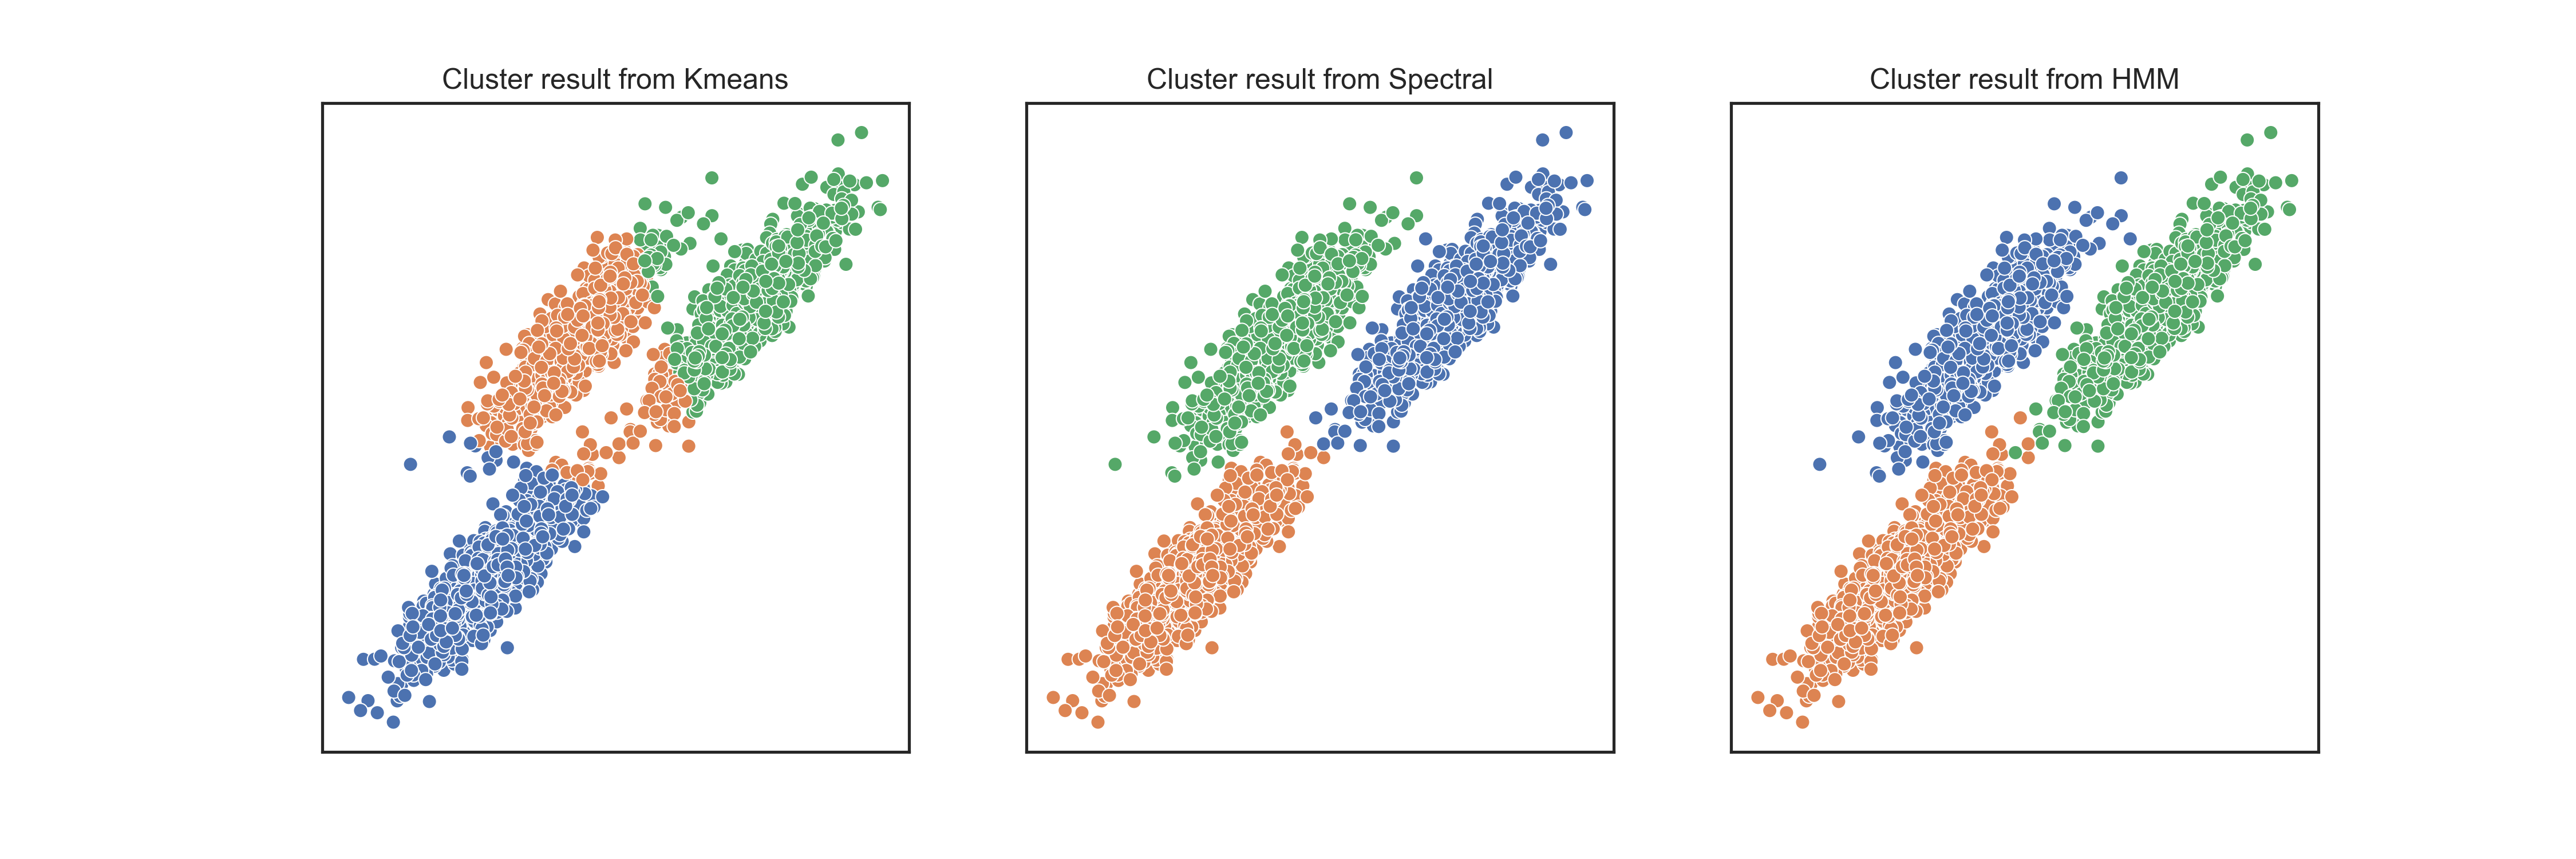
\includegraphics[width=\textwidth]{../Simu_results/sen2_clust.png}%
        \label{fig:mean and std of net34}
    \end{subfigure}\\
    \begin{subfigure}[t]{.55\columnwidth}   
        \centering 
        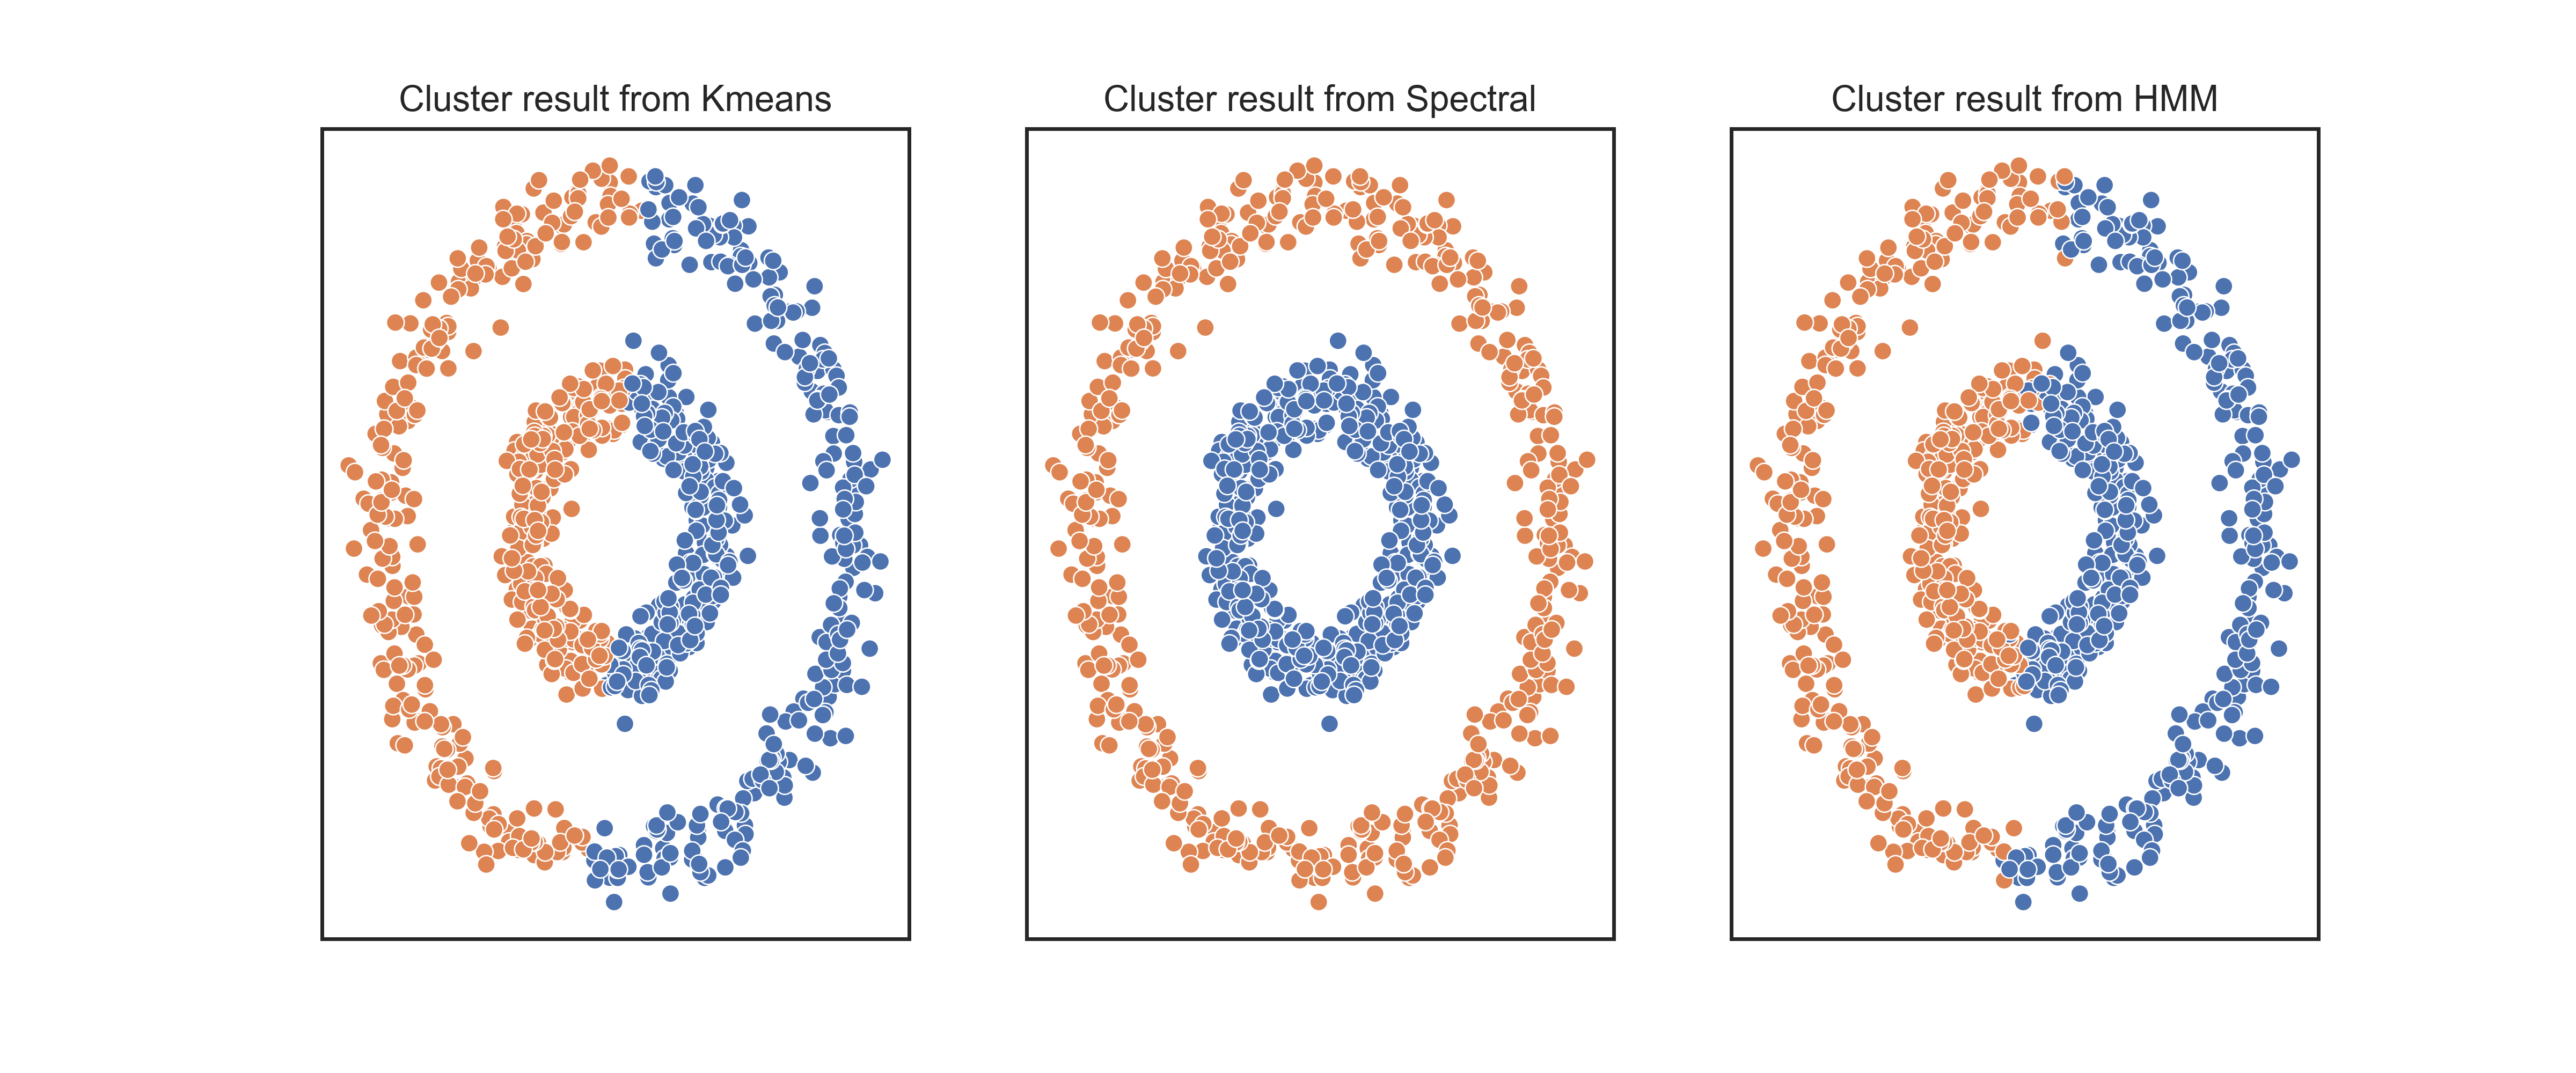
\includegraphics[width=\textwidth]{../Simu_results/sen3_clust.png}%
        \label{fig:mean and std of net34}
    \end{subfigure}
    \end{tabular}}
    \caption{{\small Clustering techniques in different scenarios}}
\end{figure}

\end{frame}


\section{Practical Example}


\begin{frame}
\frametitle{Color Quantization}


\textbf{Color quantization} reduces the number of distinct colors of an image while keeping the new image visually similar to the original one.


\begin{figure}[h!]%
    \centering
    {\renewcommand{\arraystretch}{0}
    \begin{tabular}{c@{}c}
    \begin{subfigure}[t]{.3\columnwidth}
        \centering
        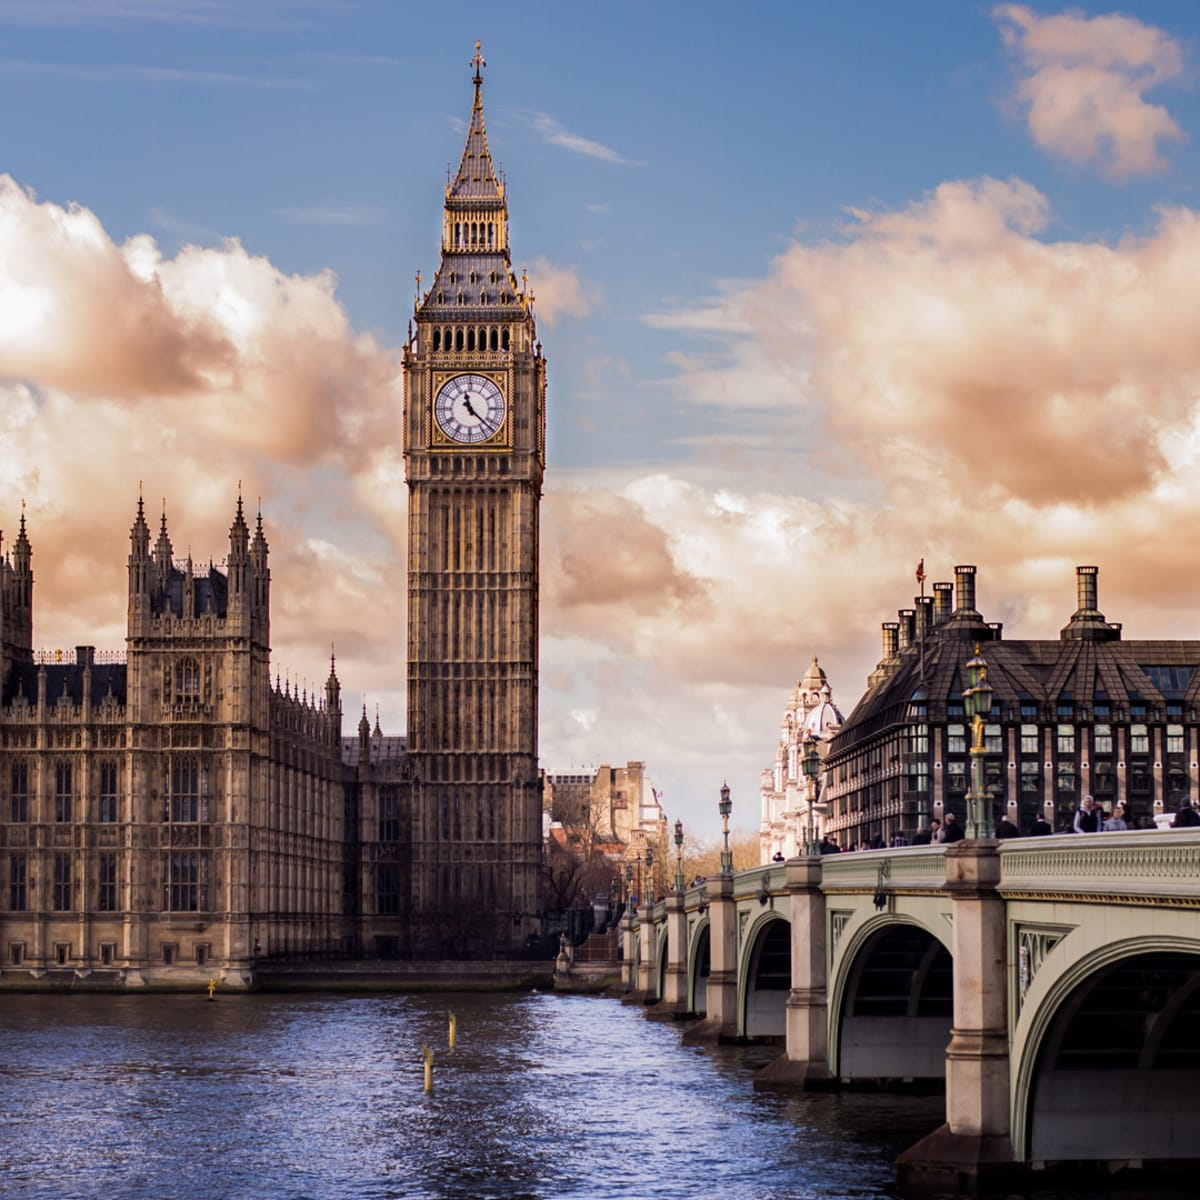
\includegraphics[width=\columnwidth]{../Cluster_results/London/London.png}%
        \subcaption{Original image}
    \end{subfigure}
    \begin{subfigure}[t]{.3\columnwidth}   
        \centering 
        \includegraphics[width=\textwidth]{../Cluster_results/London/London_kmeans_64.png}%
        \subcaption{256 code vectors}
    \end{subfigure}
    \begin{subfigure}[t]{.3\columnwidth}   
        \centering 
        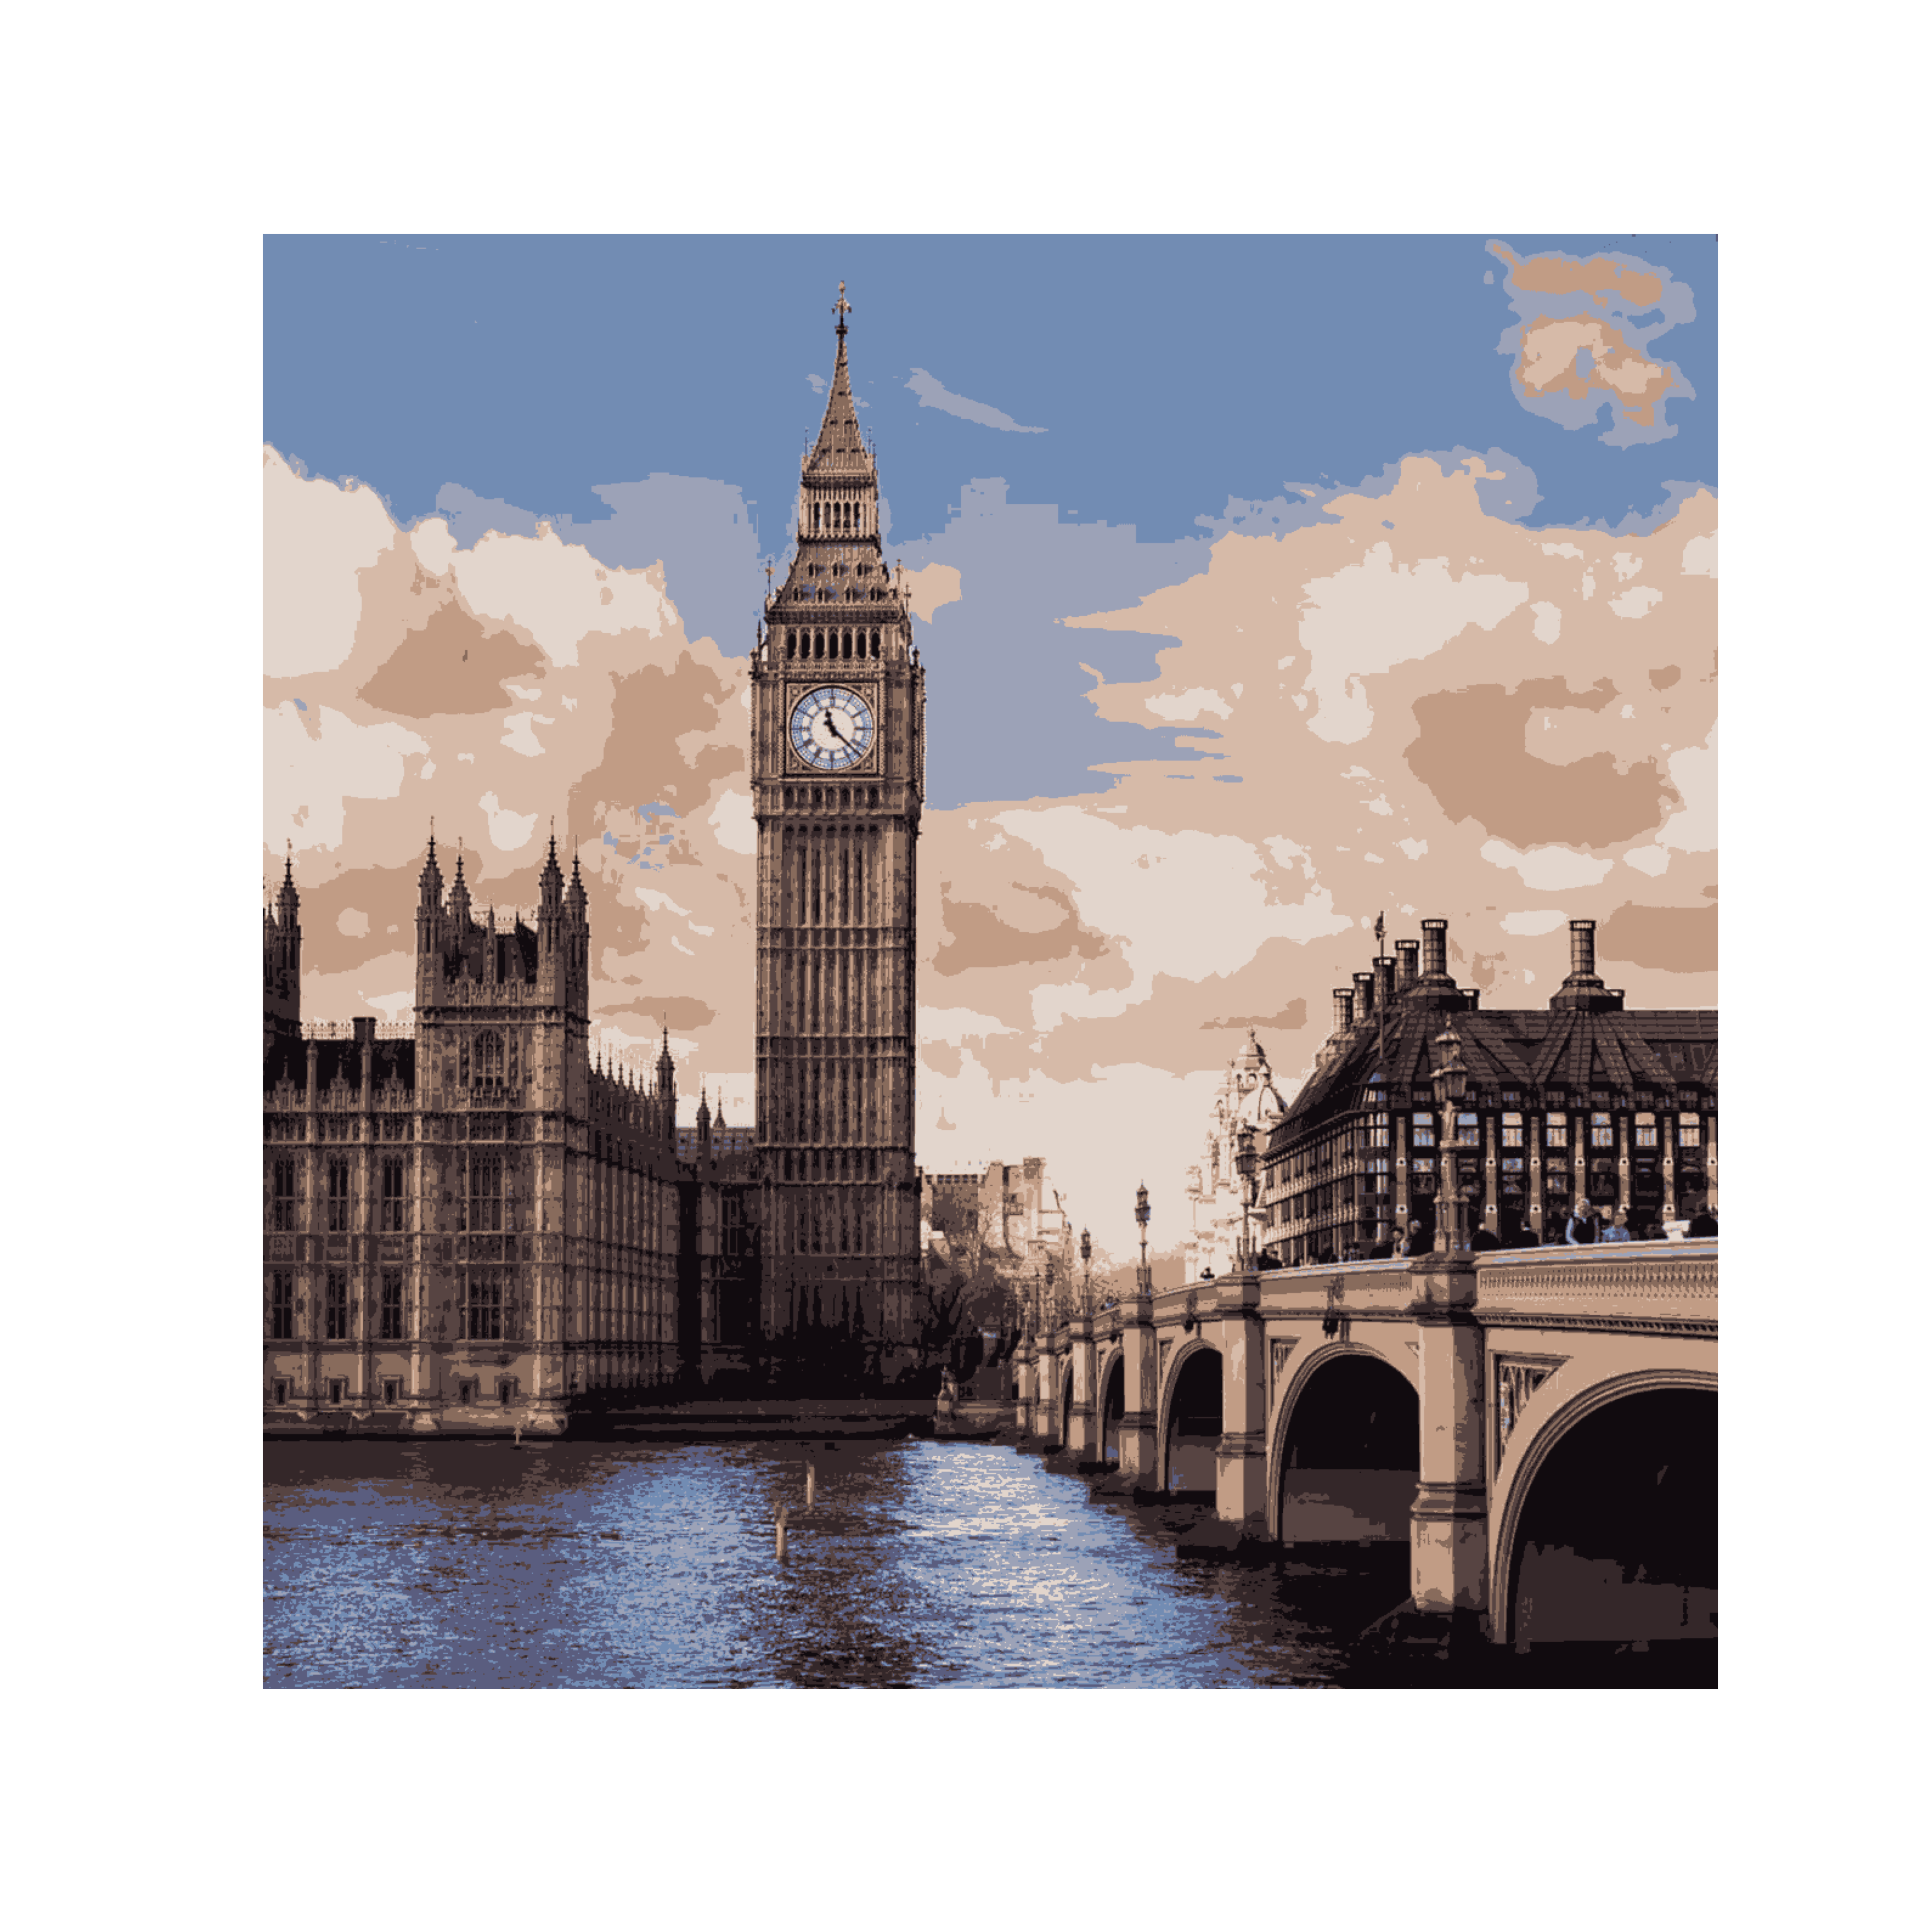
\includegraphics[width=\textwidth]{../Cluster_results/London/London_kmeans_10.png}%
        \subcaption{8 code vectors}
    \end{subfigure}
    \end{tabular}}
    \caption{Color quantization, \textit{London Bridge, London, UK}}
\end{figure}

\end{frame}

\begin{frame}
\frametitle{Color Quantization (Conti.)}

This image consists of 1200x1200 pixels: 
\begin{itemize}
	\item Each pixel is represented as 3 bytes, which occupies 24 bits of storage
	\item 256 x 256 x 256 = 16.7 million possible combination colors
	\item It requires 4 MB of storage
\end{itemize}

\

Compressed image:
\begin{itemize}
	\item with 64 code vectors requires 1.44 MB of storage
	\item with 8 code vectors only requires 540 kB of storage
\end{itemize}

\

\textbf{Trade-off between image quality and storage requirements.}

\end{frame}



\begin{frame}
\frametitle{Brain Tumor Segmentation}

\textbf{Medical image segmentation} is a task of automatically segmenting the targets of interest in a medical image. 

\begin{figure}[h!]
  \centering
  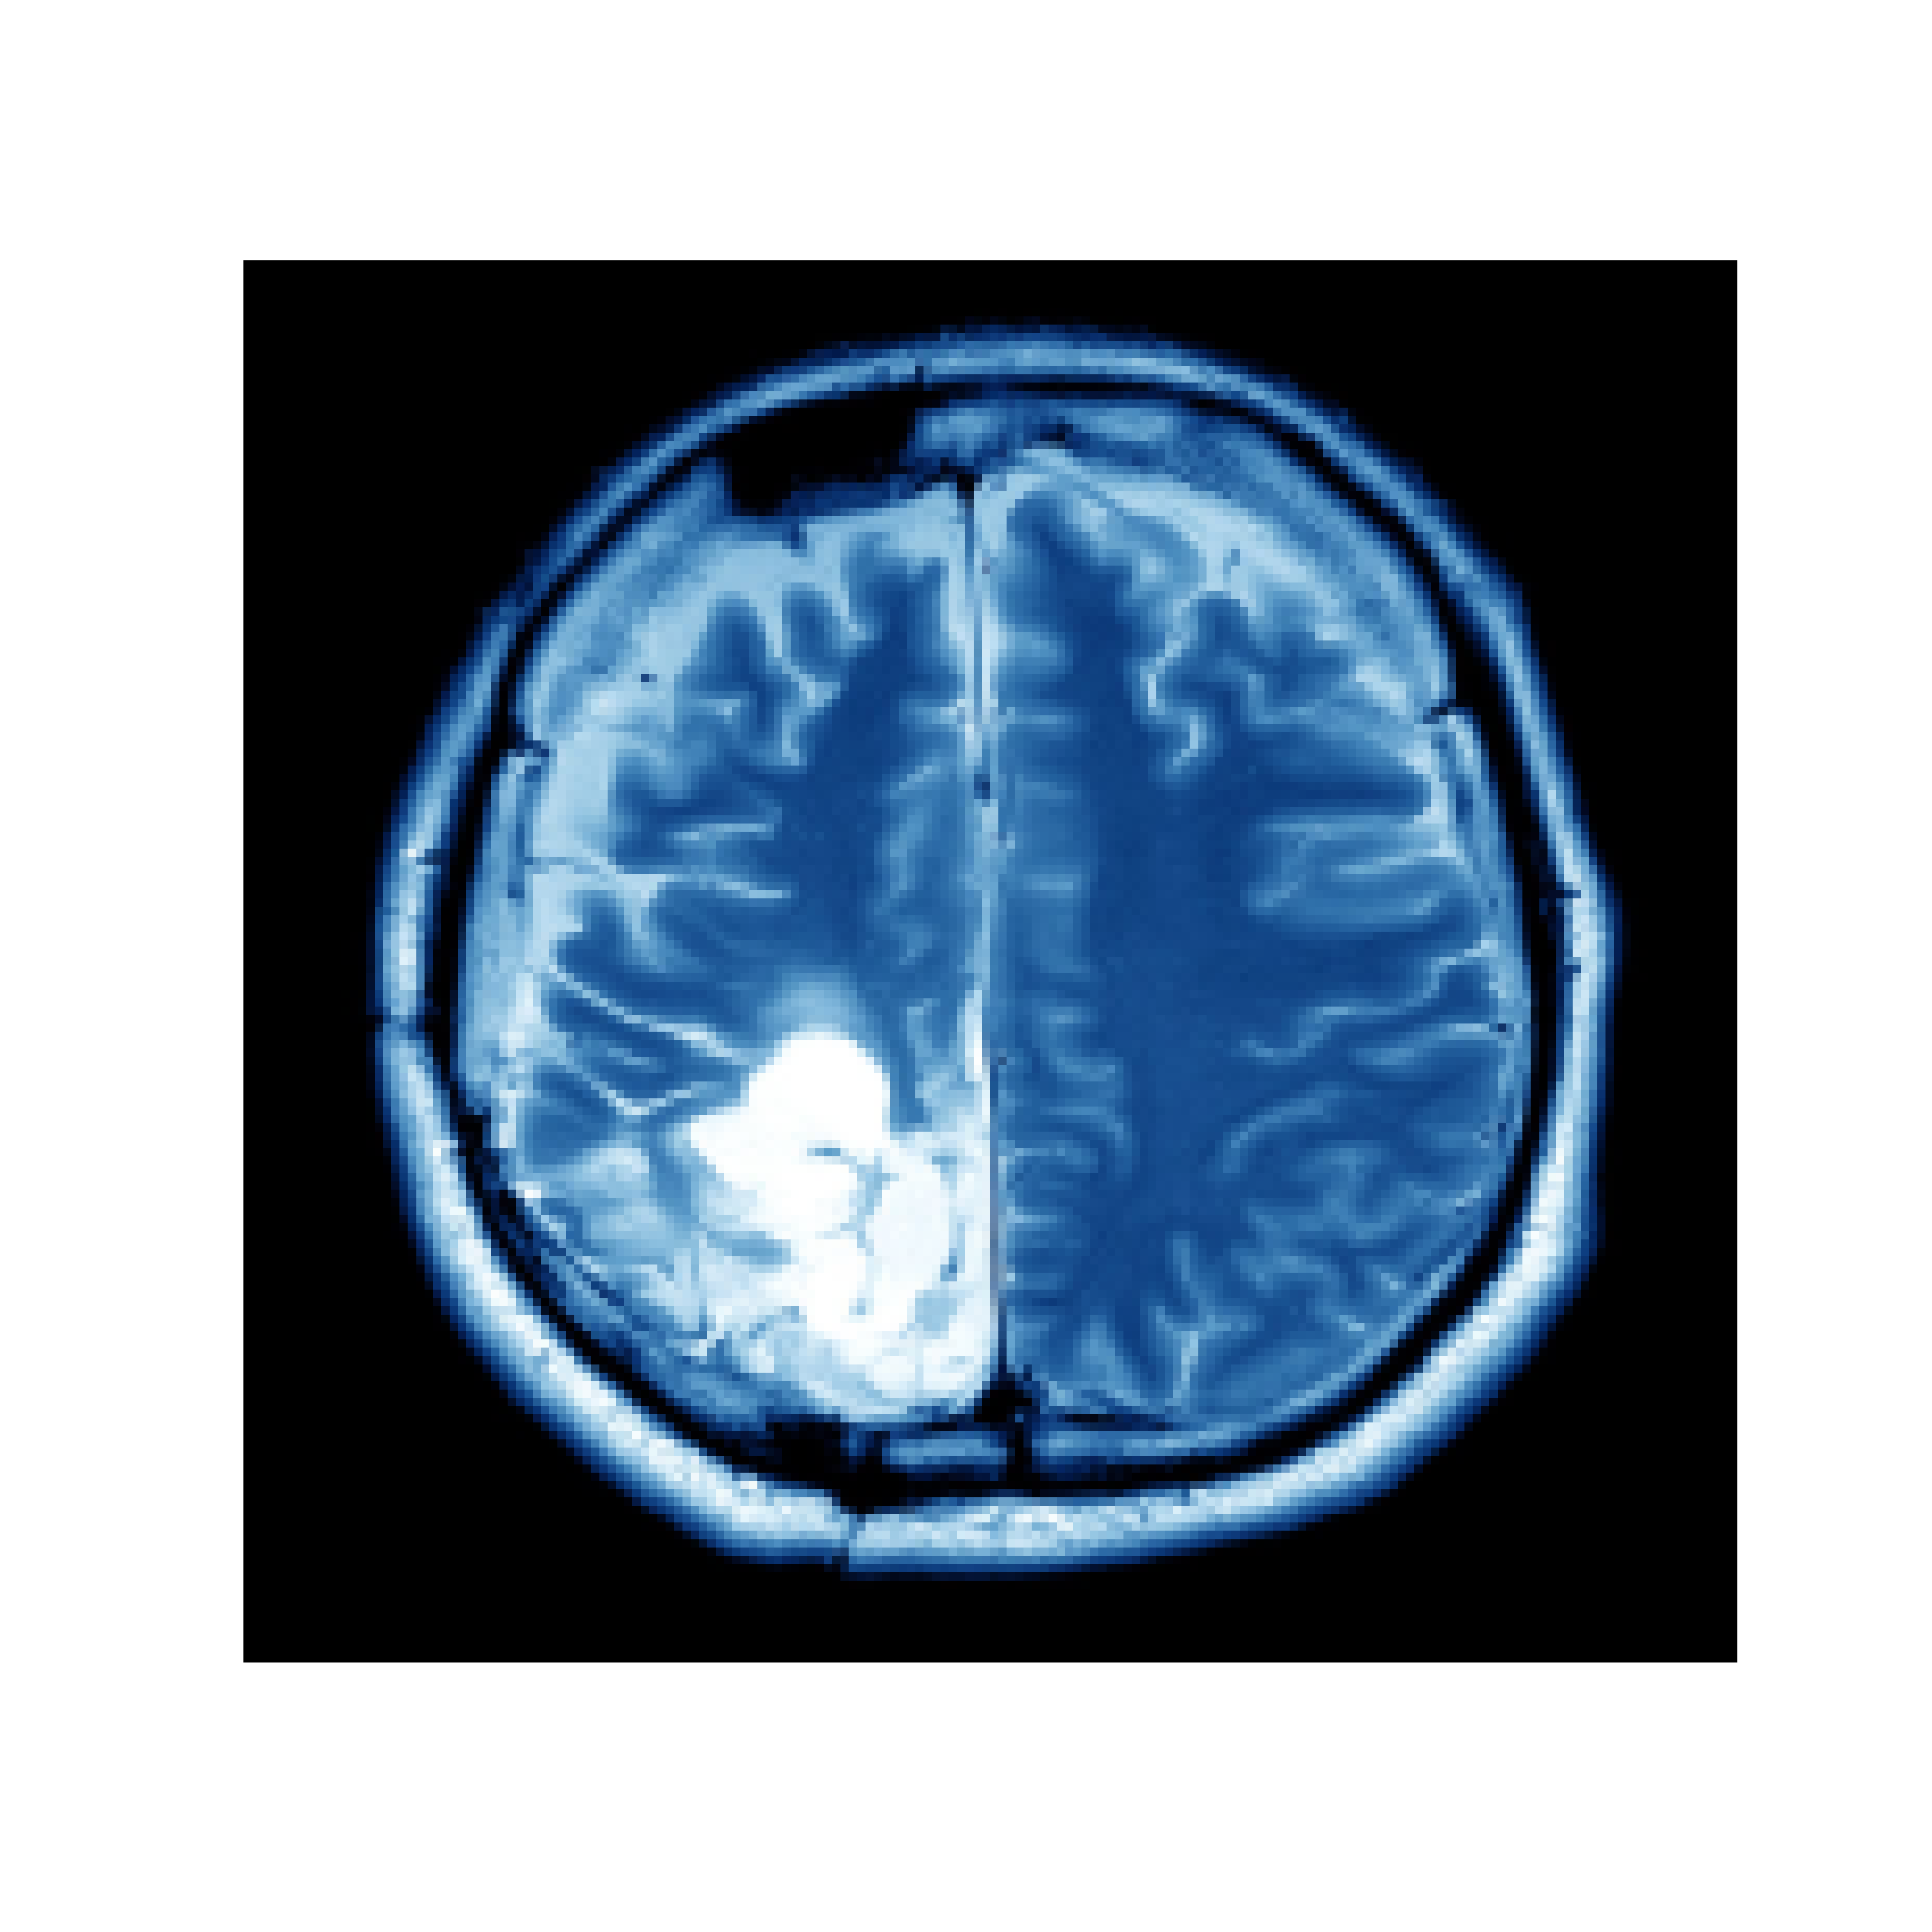
\includegraphics[width=0.4\linewidth]{../Cluster_results/MRI/MRI.png}
  \caption{\textit{tumor brain image} obtained from Stanford brain tumor center}
\end{figure}

\end{frame}


\begin{frame}
\frametitle{Brain Tumor Segmentation}

Spectral clustering outperforms the others in brain tumor segmentation.

\begin{figure}[h!]%
    \centering
    {\renewcommand{\arraystretch}{0}
    \begin{tabular}{c@{}c}
    \begin{subfigure}[t]{.3\columnwidth}
        \centering
        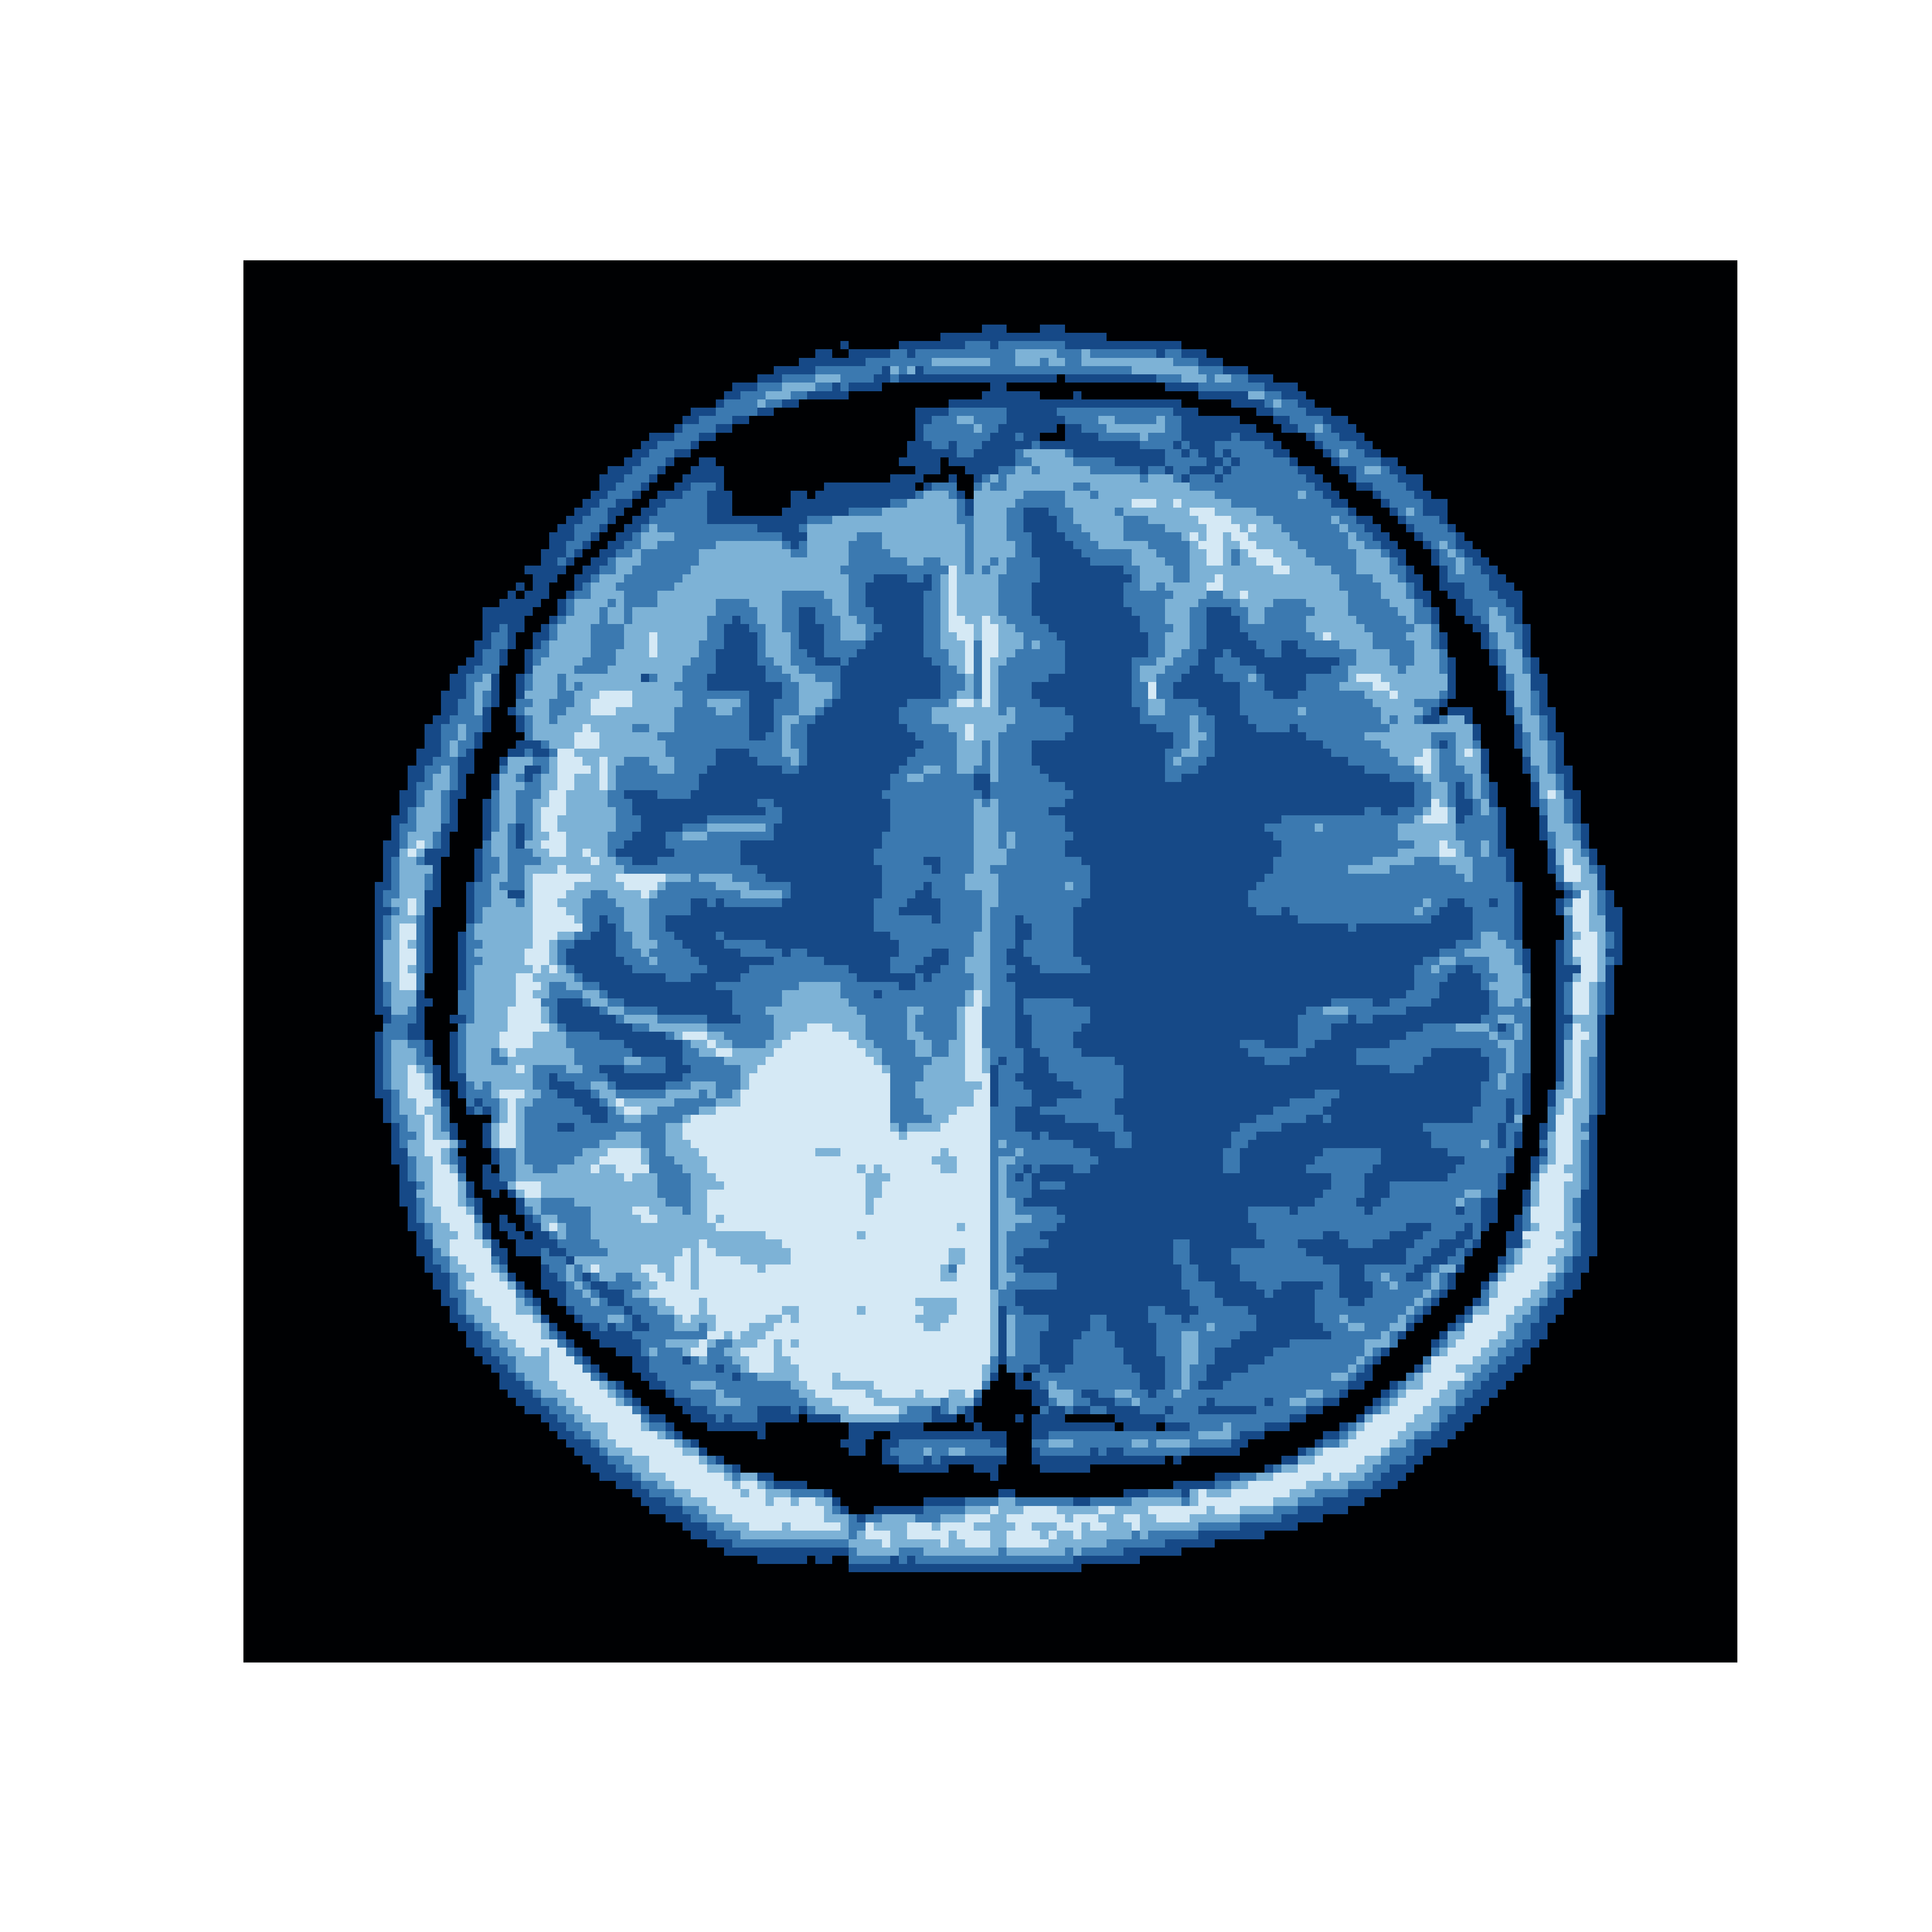
\includegraphics[width=\columnwidth]{../Cluster_results/MRI/MRI_kmeans.png}%
        \subcaption{K-means clustering}
    \end{subfigure}
    \begin{subfigure}[t]{.3\columnwidth}   
        \centering 
        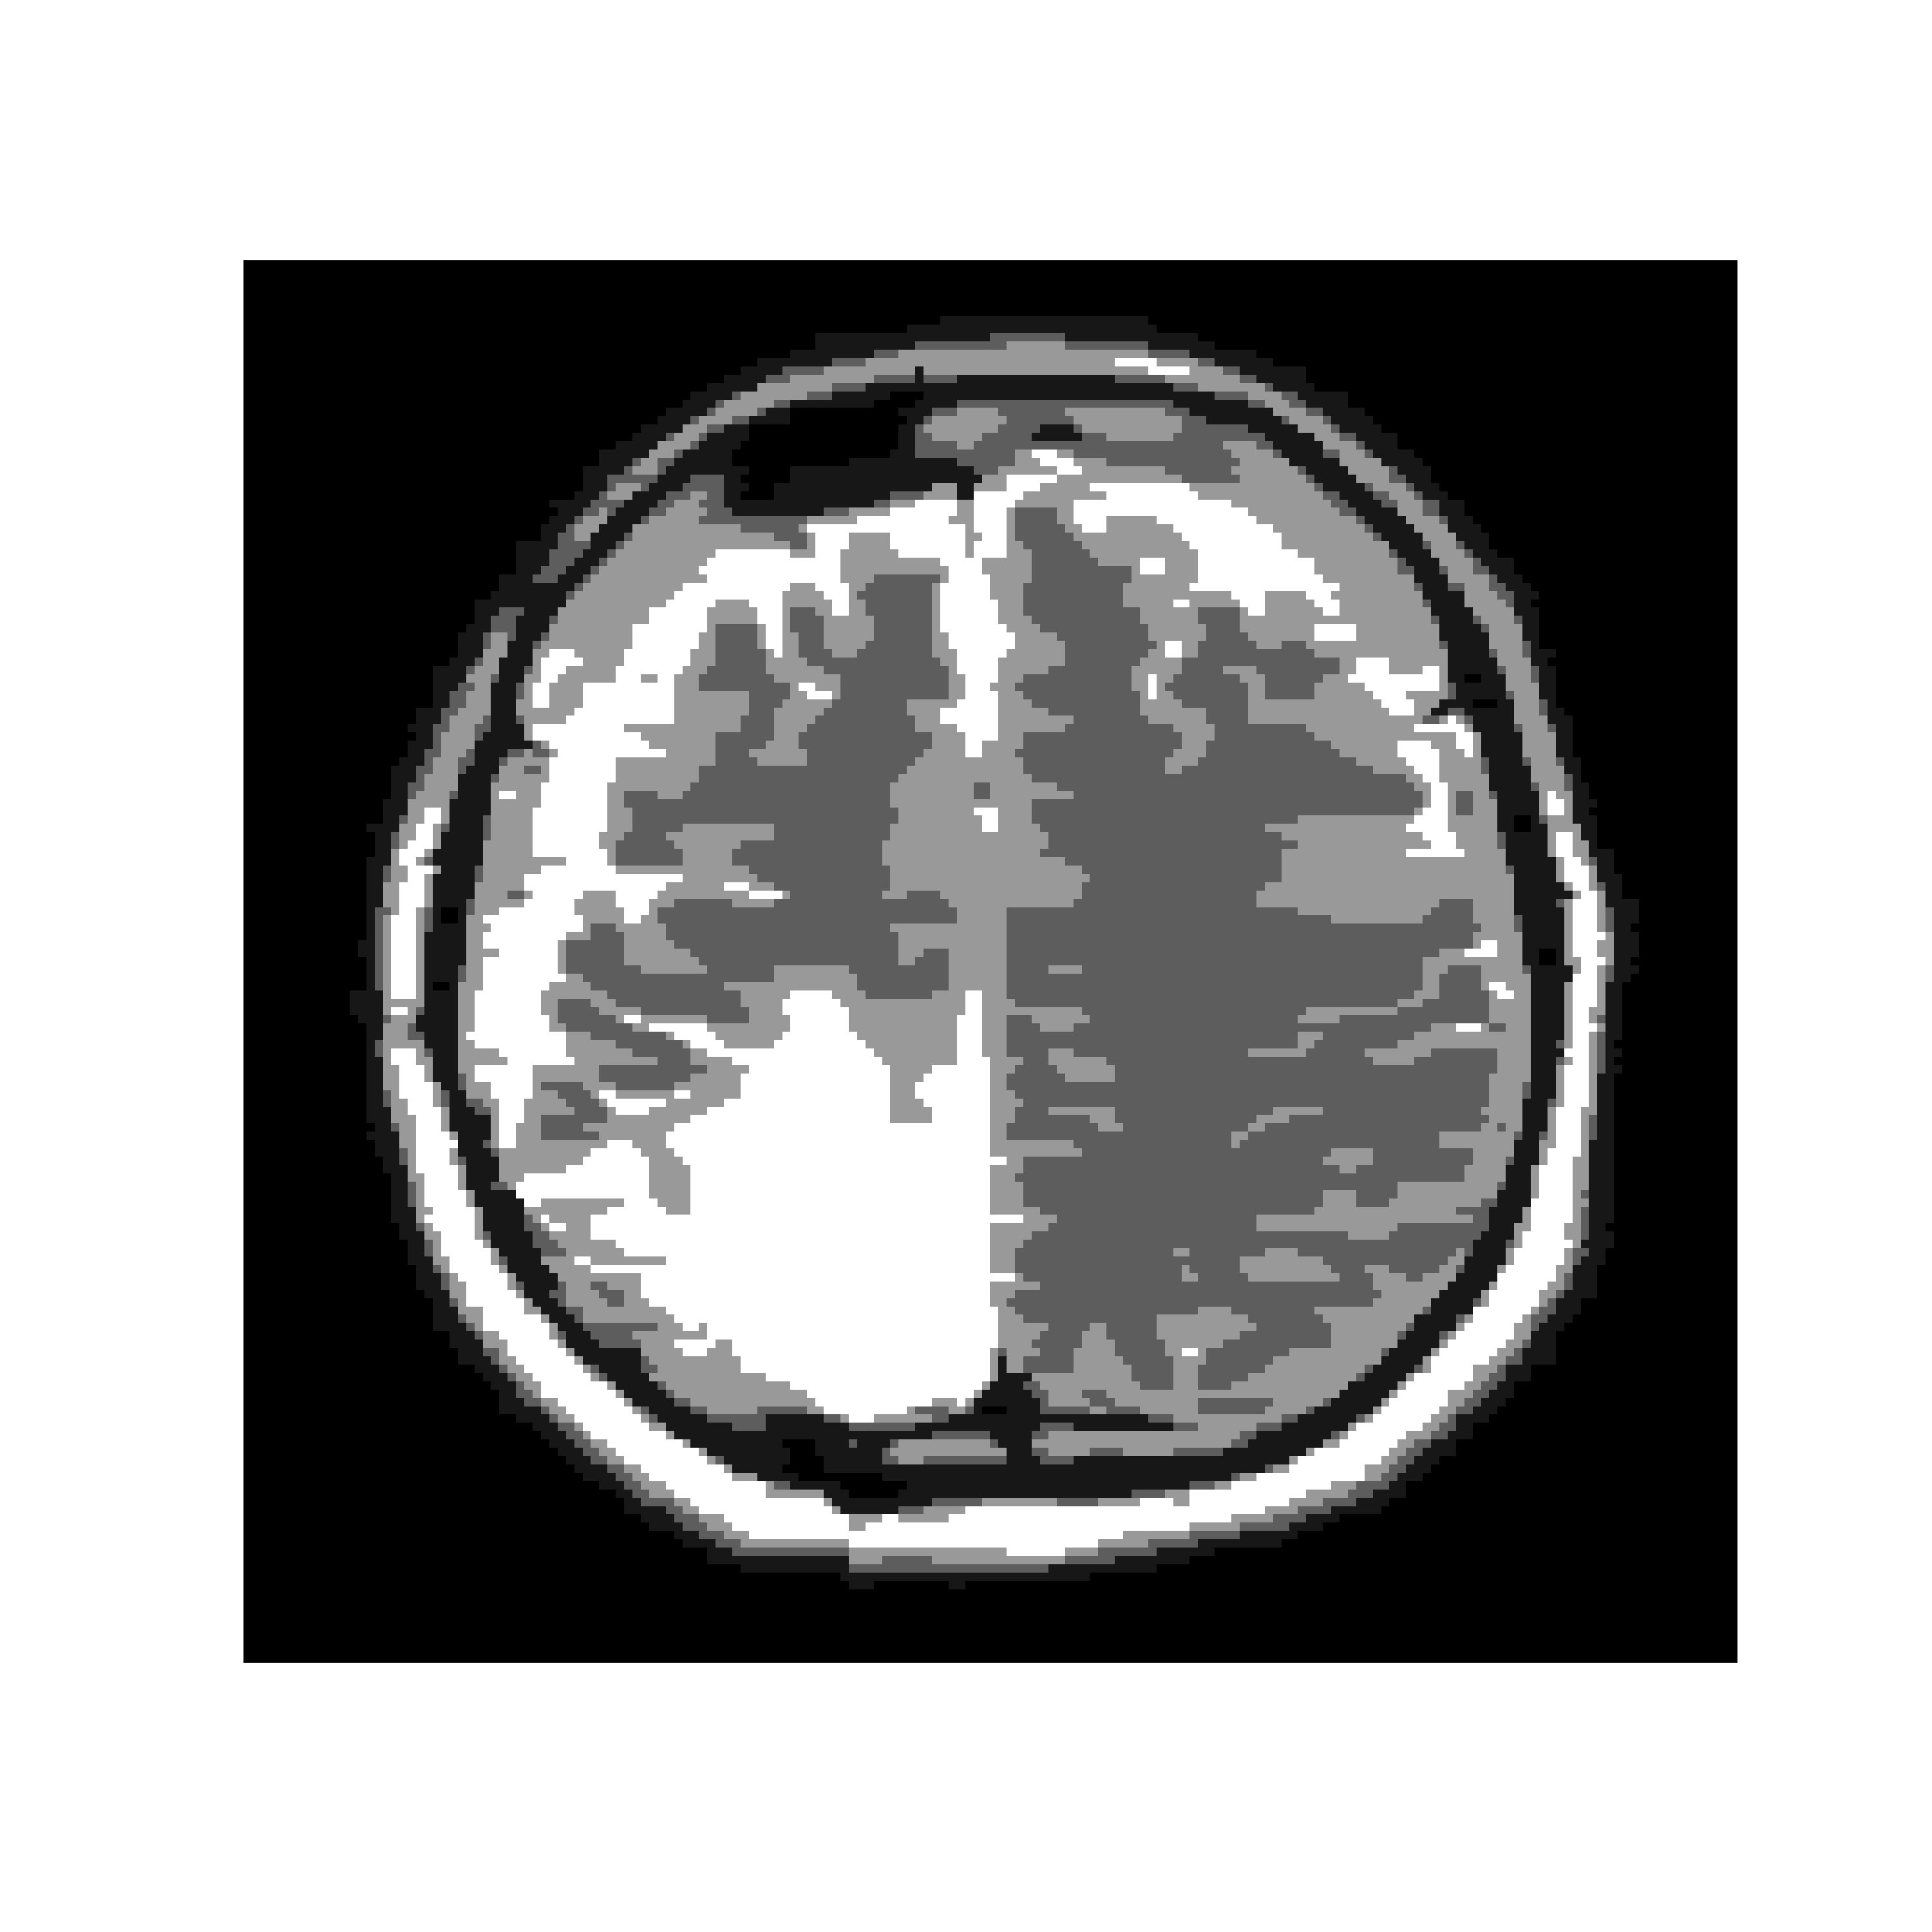
\includegraphics[width=\textwidth]{../Cluster_results/MRI/MRI_hmm.png}%
        \subcaption{HMM clustering}
    \end{subfigure}
    \begin{subfigure}[t]{.3\columnwidth}   
        \centering 
        
\includegraphics[width=\textwidth]{../Cluster_results/MRI/MRI_spec.png}%
        \subcaption{spectral clustering}
    \end{subfigure}
    \end{tabular}}
    \caption{Segmentation results}
\end{figure}


\end{frame}



\end{document}